%!TEX root = ProgCPP_ZF.tex

%TODO Beispielprojekt in Anhang

\part{Klassen}

\section{Beispielprojekt Stack}

\begin{multicols}{2}
\subsection{Stack}
\begin{minipage}{0.8\linewidth}
	\begin{itemize}
		\item Der Stack ist ein oft verwendetes Speicherkonstrukt für Daten.
		\item Bei einem Stack werden neue Elemente immer oben eingefügt.
		\item Elemente werden immer auch wieder oben weggenommen.
		\item Synonyme:
		\begin{itemize}
			\item Stapel
			\item LIFO (Last In First Out)
			\item (Kellerspeicher)
		\end{itemize}
	\end{itemize}
\end{minipage}%
\begin{minipage}{0.2\linewidth}
	\includegraphics[width=\linewidth]{images/klasse1.pdf}
\end{minipage}
\vfill\null
\columnbreak
\subsubsection{Stack - Operationen}
\begin{tabular}{ll}
	\hline 
	push() & ein neues Objekt einfügen \\ 
	\hline 
	pop() & ein Objekt entfernen \\ 
	\hline 
	isEmpty() & liefert true falls der Stack leer ist \\ 
	\hline 
	isFull() & liefert true falls der Stack voll ist \\ 
	\hline 
	init() & initialisiert einen leeren Stack \\ 
	\hline 
\end{tabular}
\end{multicols}

\subsubsection{Demo: Codebeispiel für Stack (Stack\_Datenkapsel)}
\lstinputlisting{listings/Stack_Datenkapsel/stack.h}
\lstinputlisting{listings/Stack_Datenkapsel/stack.cpp}

\subsubsection{Demo: Klasse Stack}
\begin{itemize}
	\item Stack::init() durch ctor ersetzen
	\item Verhalten bei privatem Default Ctor
	\item Verhalten bei privatem Copy Ctor
	\begin{itemize}
		\item Wenn der Copy Ctor privat deklariert wird (ohne ihn zu implementieren), dann verhindert der Compiler das Kopieren von Objekten dieser Klassen
		\item Das kann in gewissen Fällen ein durchaus erwünschtes Verhalten sein
	\end{itemize}
\end{itemize}

\begin{multicols}{2}
\subsection{Queue}
\begin{itemize}
	\item Die Queue ist ein weiteres Speicherkonstrukt für Daten.
	\item Bei einer Queue werden neue Elemente immer am Ende (tail) eingefügt.
	\item Elemente werden immer am Anfang (head) weggenommen.
	\item Synonyme:
	\begin{itemize}
		\item Warteschlange
		\item FIFO (First In First Out)
		\item Pipe
		\item Buffer (engl.)
		\item Puffer (dt.)
	\end{itemize}
\end{itemize}
\vfill\null
\columnbreak
\subsubsection{Queue - Operationen}
\begin{tabular}{lc}
	enqueue() / write() & ein neues Objekt hinzufügen \\ 
	\hline 
	dequeue() / read() & ein Objekt entfernen \\ 
	\hline 
	isFull() & liefert true falls die Queue voll ist \\ 
	\hline 
	isEmpty() & liefert true falls die Queue leer ist \\ 
	init() & initialisiert eine leere Queue \\ 
\end{tabular}
\begin{minipage}{0.7\linewidth}
	\includegraphics[width=\linewidth]{images/klasse2.pdf}
\end{minipage}
\end{multicols}

\section{Objektorientierte Programmierung}

\subsection{Prozedurale vs. Objektorientierte Sicht}
Die Objektorientierte Sicht ist meist die intuitivere Sicht der Realität als die prozedurale, da physisch existierende Objekte direkt als Objekte in einem objektorientierten Design modelliert werden können.

\clearpage
\section{Unified Modeling Language (UML)}
\href{www.uml.org}{www.uml.org}
\vspace{-\baselineskip}
\begin{multicols}{2}
\begin{minipage}{\linewidth}
	\includegraphics[width=\linewidth]{images/klasse3.pdf}
\end{minipage}
\begin{itemize}
	\item UML ist...
	\begin{itemize}
		\item \textbf{kein} Softwareprozess-Modell
		\item \textbf{kein} Lebenszyklusmodell
		\item \textbf{keine} Programmiersprache
		\item nicht ohne Redundanz
		\begin{itemize}
			\item es gibt oft mehrere Möglichkeiten, etwas zu modellieren
		\end{itemize}
		\item \textbf{kein} Softwaretool
	\end{itemize}
\end{itemize}
\vfill\null
\columnbreak
\begin{itemize}
	\item UML ist eine graphische Modellierungssprache
	\item Ziel der UML
	\begin{itemize}
		\item fortlaufendes (objektorientiertes) Modellierungskonzept für alle Software-Entwicklungsphasen
	\end{itemize}
	\item UML ist heute der de facto Standard für die Softwaremodellierung
	\item UML ist (programmier-)sprachenunabhängig
	\item UML unterstützt den gesamten Entwicklungsprozess
	\item UML integriert (fast) alle früheren Modellierungstechniken
	\begin{itemize}
		\item Datenmodellierung
		\item Prozessmodellierung
		\item Zustands- und Verhaltensmodellierung
		\item Steuerfluss-Modellierung
	\end{itemize}
\end{itemize}
\end{multicols}

\subsection{Klassenbegriff}
\begin{itemize}
	\item Eine Klasse ist eine Struktur (eine Struktur besteht nur aus Daten), die mit den Funktionen, welche auf diesen Daten arbeiten, erweitert wurde.
	\item Eine Klasse ist also eine Struktur, welche die Daten und die Funktionen auf diesen Daten in ein syntaktisches Konstrukt packt.
	\item \textbf{Die Klasse ist die Umsetzung der Datenkapsel.}
	\item Eine Klassendeklaration ist eine Typendefinition. Die "Variablen" einer Klasse werden als $"$Objekte$"$ bezeichnet.
\end{itemize}

\subsection{UML-Notation der Klasse}
\begin{itemize}
	\item Eine Klasse ist der Bauplan für Objekte.
	\item Eine Klasse besteht aus Daten (Attribute) und den Funktionen (Methoden) auf diesen Daten.
	\item Sichtbarkeit:
	\begin{itemize}
		\item[\-] +: public
		\item[\-] -: private
		\item[\-] \#: protected
	\end{itemize}
\end{itemize}

\subsection{Klasse definieren und Objekte anlegen: Syntax}
Der Name der Klasse kann fast beliebig gewählt werden.\\
\textbf{Konvention:} mit Grossbuchstaben beginnen
\noindent
\begin{minipage}{0.7\linewidth}
	\begin{lstlisting}
	class Classname	// Deklaration der Klasse
	{
		...
	};
	
	Classname obj1;				// Objekt definieren
	Classname obj2;				// Objekt definieren
	Classname* objPtr;			// Objekt-Pointer definieren
	Classname& objRef = obj1;	// Objekt-Referenz definieren
	\end{lstlisting}
\end{minipage}

\section{Zugriffsschutz bei Klassen}
\begin{itemize}
	\item Innerhalb der Klasse hat jede Methode der Klasse auf die Elemente Zugriff. (innerhalb der Klasse sind die Methoden und Attribute der Klasse "lokale Globale")
	\item Von ausserhalb der Klasse gibt es grundsätzlich keinen Zugriff auf Klassenelemente (default, d.h. wenn nichts steht)
	\item Alles, was von aussen zugreifbar sein soll, muss explizit mit \emph{public:} gekennzeichnet werden.
	\item Obwohl nicht unbedingt notwendig, werden die nach aussen nicht sichtbaren Elemente üblicherweise dennoch explizit mit \emph{private:} gekennzeichnet.
\end{itemize}

\begin{multicols}{2}
\subsection{Zugriffsschutz mit \emph{public}, \emph{protected} und \emph{private}}
\begin{description}
	\item [\emph{public:}] Elemente können innerhalb und ausserhalb der Klasse angesprochen werden.
	\begin{itemize}
		\item fast alle Methoden sind \emph{public}
		\item Attribute sollen \textbf{nie} \emph{public} sein!
	\end{itemize}
	\item [\emph{protected:}] Elemente können von innerhalb der Klasse und von abgeleiteten Klassen angesprochen werden.
	\begin{itemize}
		\item nur sparsam einsetzen
	\end{itemize}
	\item [\emph{private:}] Elemente können nur innerhalb der Klasse angesprochen werden.
	\begin{itemize}
		\item grundsätzlich für alle Attribute und für einzelne (lokale) Methoden
	\end{itemize}
\end{description}
\vfill\null
\columnbreak
\subsubsection{Üblicher Aufbau einer Klassenschnittstelle}
\vspace{-\baselineskip}
\begin{minipage}{\linewidth}
	\begin{lstlisting}
	class Classname	// Klassendeklaration
	{
		public:
			...
		protected:
			...
		private:
			...
	};
	\end{lstlisting}
\end{minipage}
\begin{achtung}
	Strichpunkt nicht vergessen!
\end{achtung}
\end{multicols}

\subsection{Information Hiding}
\begin{itemize}
	\item Klassen exportieren generell ausschliesslich Methoden.
	\item[\-] Alle Daten sind im Innern (private-Abschnitt) verborgen, der Zugriff erfolgt über die so genannten Elementfunktionen.
	\item Jede Klasse besteht damit aus zwei Dateien, der Schnittstellendatei (.h) und der Implementierungsdatei (.cpp).
\end{itemize}

\section{Beispiel einer Klasse: Rechteck (Rectangle)}
\begin{multicols}{2}
\begin{itemize}
	\item Welche Attribute besitzt ein Rechteck?
	\begin{itemize}
		\item Länge a
		\item Breite b
	\end{itemize}
	\item Welche Funktionen (Methoden) sollen möglich sein?
	\begin{itemize}
		\item a und b setzen
		\item a und b abfragen
		\item Flächeninhalt abfragen
	\end{itemize}
\end{itemize}
\columnbreak
\includegraphics[width=0.6\linewidth]{images/klasse4.pdf}
\end{multicols}

\subsection{Klassendeklaration}
\vspace{-\baselineskip}
\begin{minipage}{0.4\linewidth}
	\lstinputlisting{listings/rectangle.h}
\end{minipage}

\begin{multicols}{2}
\subsection{Klassendefinition}
\vspace{-\baselineskip}
\begin{minipage}{\linewidth}
	\lstinputlisting{listings/rectangle.cpp}
\end{minipage}
\vfill\null
\columnbreak
\subsection{Klassendefinition direkt}
\vspace{-\baselineskip}
\begin{minipage}{\linewidth}
	\lstinputlisting{listings/rectangle_direkt.h}
\end{minipage}
\begin{hinweis}
	Ist ok bei sehr kurzen Methoden. Verletzt Information Hiding, Methoden sind jedoch implizit inline.
\end{hinweis}
\end{multicols}

\subsection{Klassenschnittstelle}
Die Schnittstelle einer Klasse sollte minimal und vollständig sein. Vollständig in dem Sinne, dass Benutzer der Klasse alle sinnvollen Aktionen ausführen können. Minimal wiederum bedeutet, dass das Klassen-Interface so klein wie möglich sein sollte.

\section{Elementfunktionen}
\begin{itemize}
	\item Sind Funktionen, die in der Schnittstelle der Klasse spezifiziert sind.
	\item Elementfunktionen haben vollen Zugriff auf alle Klassenelemente (auch auf solche, die mit \emph{private} gekennzeichnet sind).
	\item Auf Elementfunktionen kann nur unter Bezugnahme auf ein Objekt der Klasse, bzw. mit dem Scope-Operator (\emph{::}) zugegriffen werden.
	\item Elementfunktionen sollen prinzipiell in der Implementierungsdatei (\emph{.cpp}) implementiert werden. Dem Funktionsnamen muss dabei der Klassenname gefolgt von \emph{::} vorgestellt werden.
\end{itemize}

\subsection{Klassifizierung von Elementfunktionen}
\begin{itemize}
	\item Konstruktoren/Destruktoren
	\begin{itemize}
		\item Konstruktor: erzeugen eines Objekts
		\item Destruktor: vernichten, freigeben eines Objekts
	\end{itemize}
	\item Modifikatoren
	\begin{itemize}
		\item ändern den Zustand eines Objekts (Attribute ändern)
	\end{itemize}
	\item Selektoren
	\begin{itemize}
		\item greifen nur lesend auf ein Objekt zu (immer const definieren!)
		\item Beispiel:
		\item[\-] \vspace{-\baselineskip} \begin{minipage}{0.4\linewidth}
\begin{lstlisting}
bool Stack::isEmpty() const;
\end{lstlisting}
	\end{minipage}
	\end{itemize}
	\item Iteratoren
	\begin{itemize}
		\item Erlauben, auf Elemente eines Objekts in einer definierten Reihenfolge zuzugreifen
	\end{itemize}
\end{itemize}

\subsection{inline-Elementfunktionen}
\begin{itemize}
	\item Elementfunktionen, die innerhalb der Deklaration der Klassenschnittstelle (im .h-File) implementiert sind, werden als (implizite) inline-Funktionen behandelt.
	\begin{itemize}
		\item Implizite inline-Funktionen verletzen das Information Hiding Prinzip und sollten deshalb vermieden werden!
	\end{itemize}
	\item Elementfunktionen können in der Klassenimplementation explizit mit dem Schlüsselwort \emph{inline} gekennzeichnet werden.
	\item Jedoch: die impliziten \emph{inline}-Funktionen sind die Funktionen, die garantiert immer \emph{inline} verwendet werden (mit einigen wenigen Ausnahmen).
\end{itemize}

\subsection{\emph{const} - Elementfunktionen}
\begin{itemize}
	\item Elementfunktionen, die den Zustand eines Objekts nicht ändern (Selektoren) sollen explizit mit dem Schlüsselwort \emph{const} gekennzeichnet werden.
	\item Das Schlüsselwort \emph{const} muss sowohl im Prototypen als auch in der Implementierung geschrieben werden.
	\item Beispiel:
	\item[\-] \vspace{-\baselineskip}
	\begin{minipage}{0.4\linewidth}
\begin{lstlisting}
bool Stack::isEmpty() const;
...
bool Stack::isEmpty() const
{
	return top == 0;
}
\end{lstlisting}
	\end{minipage}
\end{itemize}
Um zu verhindern, dass \emph{const}-Objekte über den $"$Umweg$"$ von Elementfunktionen verändert werden, dürfen $"$normale$"$ Elementfunktionen nicht auf \emph{const}-Objekte angewandt werden.
\noindent
\begin{minipage}{0.9\linewidth}
\begin{lstlisting}
class Stack
{
	public:
		int pop();
		bool isEmpty() const;
	private:
		...
};
...
void fooReadOnly(const Stack& s)
{
	bool b = s.isEmpty();	// ok. s ist const, isEmpty() ist auch const
	int i = s.pop();	// Fehler. s ist const, pop() nicht!
}
\end{lstlisting}
\end{minipage}

\begin{hinweis}
Damit mit \emph{const}-Objekten überhaupt etwas gemacht werden kann, müssen die Elementfunktionen, welche die Attribute nicht verändern, konsequent mit \emph{const} gekennzeichnet werden.
\end{hinweis}

\subsection{\emph{mutable}-Attribut}
Ein Datenelement, das nie \emph{const} werden soll (auch nicht bei \emph{const}-Elementfunktionen), kann mit \emph{mutable} gekennzeichnet werden.
\vspace{-\baselineskip}
\begin{minipage}{0.85\linewidth}
\begin{lstlisting}
class Stack
{
	public:
		int pop();
		int peek() const; // read-only, liest nur das oberste Element
		bool isEmpty() const;
	private:
		int elem[maxElems]; // Array fuer Speicherung des Stacks
		int top; // Arrayindex des naechsten freien Elements
		mutable bool error; // true: Fehler passiert
		// mutable: auch const-Methoden koennen dieses Attribut setzen
};

int Stack::peek() const
{
	error = top == 0; // auch in const-Methode setzbar
	if (!error)
		return elem[top-1];
	else
		return elem[top];
}
\end{lstlisting}
\end{minipage}

\section{Konstruktoren/Destruktoren}

\subsection{\emph{this}-Pointer}
Der \emph{this}-Pointer ist ein Pointer auf das eigene aktuelle Objekt, welches eine Elementfunktion (Methode) aufgerufen hat.
\vspace{-\baselineskip}
\begin{minipage}{\linewidth}
	\begin{lstlisting}
	const AnyClass& AnyClass::aMethod(const AnyClass& obj)
	{
		this->anyFoo();	// Aufruf einer Methode ueber this
				// 'this' ist hier unnoetig, da Methode implizit mit aktuellem
				// Objekt ausgefuehrt wird
		if(this == &obj)// testen, ob eigene Adresse gleich der Adresse von obj ist
			...
		return *this;	// eigenes Objekt zurueckgeben
	}
	\end{lstlisting}
\end{minipage}

\subsection{\emph{friend}-Elemente}
\begin{itemize}
	\item \emph{friend} - Jede Klasse kann andere Klassen oder Funktionen "zum Freund" erklären. Dadurch werden die Zugriffsregeln durchbrochen.
	\item Jeder \emph{friend} darf auf \textbf{alle} Elemente der Klasse zugreifen.
\end{itemize}
\begin{achtung}
	\emph{friends}, insbesondere \emph{friend}-Klassen, können ein Anzeichen für schlechtes Design sein. Sie durchbrechen wichtige Prinzipien der objektorientierten Programmierung.
	\textbf{Die Verwendung von \emph{friend} sollte daher weitgehend unterbleiben.}
	Für ausgewählte Anwendungen kann damit jedoch sehr elegant programmiert werden (siehe Kap.\ref{sec:operator overloading}).
\end{achtung}

\subsection{\emph{static}-Klassenelemente}
\begin{itemize}
	\item Grundsätzlich besitzt jedes Objekt einer Klasse seine eigene private Instanz aller Attribute einer Klasse.
	\item Wenn ein Attribut mit \emph{static} gekennzeichnet wird, dann teilen sich alle Objekte dieser Klasse eine eigene Instanz dieses Attributs, d.h. ein statisches Attribut ist nur einmal für alle Objekte einer Klasse im Speicher vorhanden.
	\item \emph{static}-Elemente befinden sich ausserhalb eines Objektkontextes.
	\item \emph{static}-Elemente können auch über den Klassennamen angesprochen werden (da sie sich im Kontext einer Klasse befinden).
\end{itemize}

\subsubsection{Syntax}
\vspace{-\baselineskip}
\begin{minipage}{\linewidth}
\begin{lstlisting}
class T
{
	...
	static int nrOfObjects = 34;	// Initialisierung ist ab C++03
					// in der Deklaration nicht mehr erlaubt!
	static int nrOfObjects;		// Korrekt
};

static int T::nrOfObjects;	// Die Initialisierung kann in der Definition (.cpp)
			// erfolgen. Das Schluesselwort static muss hier weggelassen werden.
int T::nrOfObjects = 34;	// Definition (ist notwendig)

T myT;
myT.nrOfObjects++;		// Zugriff ueber Objekt (falls public)
T::nrOfObjects++;		// Zugriff ueber Klasse (falls public)
\end{lstlisting}
\end{minipage}

\subsection{Konstruktor (Constructor, Ctor)}
Aufgaben:
\begin{itemize}
	\item Die Neugründung einer Objekts einer Klasse.
	\item Das $"$saubere$"$ initialisieren des Objekts, d.h. \textbf{alle} Attribute des Objekts müssen auf einen definierten Wert gesetzt werden.
	\item Der Konstruktor hat in C++ denselben Namen wie die Klasse, hat keinen Rückgabetyp (auch nicht void) und kann überladen werden.\\
	\vspace{-\baselineskip}
	\begin{minipage}{0.55\linewidth}
\begin{lstlisting}
Stack::Stack();	// (Default-)Konstruktor
\end{lstlisting}
	\end{minipage}
\end{itemize}

\subsubsection{Aufruf}
\label{sec:aufruf}
\begin{itemize}
	\item Der Konstruktor soll nie explizit aufgerufen werden.
	\item Der Konstruktor wird vom System automatisch (implizit) aufgerufen, wenn ein Objekt erzeugt wird.\\
	\vspace{-\baselineskip}
	\begin{minipage}{0.15\linewidth}
\begin{lstlisting}
Stack s;
\end{lstlisting}
	\end{minipage}
	\item Wenn durch den \emph{new}-Operator Speicher angefordert \textbf{und} erhalten wird, dann wird der Konstruktor vom System ebenfalls automatisch aufgerufen.\\
	\vspace{-\baselineskip}
	\begin{minipage}{0.3\linewidth}
\begin{lstlisting}
Stack* pS = new Stack;
\end{lstlisting}
	\end{minipage}
\end{itemize}

\subsection{Welcher Konstruktor wird wann aufgerufen?}
\begin{itemize}
	\item Ein Konstruktor wird ausschliesslich dann aufgerufen, wenn ein neues Objekt erzeugt wird.
	\item Wenn feststeht, dass ein Konstruktor benötigt wird, muss man sich noch überlegen, welcher der allenfalls überladenen Konstruktoren aufgerufen wird.
\end{itemize}

\subsection{Default-Konstruktor}
\begin{itemize}
	\item Der Default-Konstruktor ist der Konstruktor ohne Parameter.
	\item Er wird immer aufgerufen, wenn bei der Objekterzeugung keine Parameter mitgegeben werden.
	\item Der Default-Konstruktor kann selbst definiert werden.
	\begin{itemize}
		\item Das ist insbesondere dann notwendig, wenn innerhalb des Objekts Speicher dynamisch alloziert werden muss (bei der Objekterzeugung).
	\end{itemize}
	\item Der Default-Konstruktor wird vom System automatisch erzeugt, wenn für eine Klasse kein Konstruktor explizit definiert ist.
\end{itemize}

\begin{multicols}{2}
\subsubsection{Beispiel: Klasse TString (nach Lippman)}
\vspace{-\baselineskip}
\begin{minipage}{\linewidth}
	\begin{lstlisting}
	class TString
	{
		public:		
			TString();	// Default-Konstruktor
			int getLen() const;
		private:
			int len;
			char* str;
	};
	\end{lstlisting}	
\end{minipage}
\vfill\null
\columnbreak
\subsubsection{Implementation von TString::TString()}
\vspace{-\baselineskip}
\begin{minipage}{\linewidth}
	\begin{lstlisting}
	// mit Anweisungen
	TString::TString()
	{
		len = 0;
		str = 0;
	}
	
	// mit Initialisierungsliste (ist besser)
	TString::TString()
		: len(0), str(0)
	{
	}
	\end{lstlisting}
\end{minipage}
\begin{hinweis}
	Objektinitialisierungen werden, sofern dies möglich ist, über die Initialisierungsliste durchgeführt. (Effizienzgründe)
\end{hinweis}
\end{multicols}

\subsubsection{Überladen von Konstruktoren}
\begin{itemize}
	\item Der Default-Konstruktor wird implizit aufgerufen mit:\\
	\vspace{-\baselineskip}
	\begin{minipage}{\linewidth}
\begin{lstlisting}
TString str;
\end{lstlisting}
	\end{minipage}
	\item Ein TString-Objekt soll auch z.B: mit folgenden Anweisungen gegründet werden können:\\
	\vspace{-\baselineskip}
	\begin{minipage}{\linewidth}
\begin{lstlisting}
	TString str1 = "Hello";								// implicit call
	TString str2 = TString("Guten Morgen");	// explicit call
\end{lstlisting}
	\end{minipage}
	\item Dazu bedarf es anderer (überladener) Konstruktoren.
\end{itemize}

\begin{multicols}{2}
\subsubsection{Erweiterung der Klasse TString}
\vspace{-\baselineskip}
\begin{minipage}{\linewidth}
\begin{lstlisting}
class TString
{
	public:
		TString();	// Default-Konstruktor
		TString(const char* p);
		int getLen() const;
	private:
		int len;
		char* str;
};
\end{lstlisting}
\end{minipage}
\vfill\null
\columnbreak
Implementation:\\
\vspace{-\baselineskip}
\begin{minipage}{\linewidth}
\begin{lstlisting}
TString::TString(const char* p)
{
	if(p==0)
	{
		len = 0;
		str = 0;
	}
	else
	{
		len = strlen(p);
		str = new char[len+1];
		memcpy(str, p, len+1);
	}
}
\end{lstlisting}
\end{minipage}
\begin{hinweis}
	Hier geht Initialisierungsliste nicht.
\end{hinweis}
\end{multicols}

\subsubsection{Konstruktoren und Function Casts}
\begin{itemize}
	\item Konstruktoren mit nur einem Parameter können dazu verwendet werden, ein Objekt vom Typ T aus einem anderen Objekt zu erzeugen (Typumwandlung).
	\item Beispiel:
	\item[\-] TString soll so erweitert werden, dass dem Konstruktor eine ganze Zahl übergeben wird und dieser daraus den entsprechenden String erzeugt.\\
	\vspace{-\baselineskip}
	\begin{minipage}{\linewidth}
\begin{lstlisting}
TString::TString(int number);

// explicit call:
TString str1 = TString(12345);	// erzeugt "12345"
\end{lstlisting}
	\end{minipage}
	\item Die implicit calls (bei Ctors mit einem Parameter)\\
	\vspace{-\baselineskip}
	\begin{minipage}{\linewidth}
\begin{lstlisting}
// implicit calls
TString str2 = 12345;			// erzeugt "12345"
str2 = 789;		// erzeugt temporaeres Objekt "789" und weist dieses str2 zu
\end{lstlisting}
	\end{minipage}
	\item[\-] sind gelegentlich nicht erwünscht.
	\item Wenn der Konstruktor mit explicit gekennzeichnet wird, kann dieser Ctor nicht mehr implizit, sondern nur explizit aufgerufen werden.
	\begin{minipage}{\linewidth}
\begin{lstlisting}
explicit TString::TString(int number);

TString str1 = TString(12345);	// ok (explicit)
TString str2 = 12345;						// nicht erlaubt (implicit call)
str2 = 78;											// nicht erlaubt (implicit call)
str1 = 567;											// nicht erlaubt (implicit call)
\end{lstlisting}
	\end{minipage}
\end{itemize}

\subsubsection{Erweiterung der Klasse TString mit explicit-Ctor}
\vspace{-\baselineskip}
\begin{minipage}{0.5\linewidth}
\begin{lstlisting}
class TString
{
	public:
		TString();		// Default-Konstruktor
		TString(const char* p);
		explicit TString(int number);
		int getLen() const;
	private:
		int len;
		char* str;
};
\end{lstlisting}
\end{minipage}

\subsubsection{Copy-Konstruktor}
\begin{itemize}
	\item Der Copy-Konstruktor wird dazu verwendet, Objekte zu kopieren.
	\item Der Copy-Konstruktor erhält als Parameter immer eine konstante Referenz auf ein Objekt der Klasse. Für TString sieht er wie folgt aus:\\
	\vspace{-\baselineskip}
	\begin{minipage}{\linewidth}
\begin{lstlisting}
TString(const TString& s);		// Copy-Konstruktor

// welche Konstruktoren werden aufgerufen?
TString str1("Hello World");	// normaler Konstruktor TString(const char* p)
TString str2 = str1;		// Copy-Konstr. (Initialisierung, nicht Zuweisung!)
TString str3(str1);						// Copy-Konstruktor
\end{lstlisting}
	\end{minipage}
\end{itemize}

\subsubsection{Copy-Konstruktor wird automatisch aufgerufen, wenn...}
\begin{itemize}
	\item ein Objekt erzeugt und mit einem anderen Objekt derselben Klasse initialisiert wird.
	\item ein Objekt als Wertparameter (\emph{by value}) an eine Funktion übergeben wird (nicht aber bei Referenzierungsparametern $\rightarrow$ wichtig!).
	\item ein Objekt \emph{by value} als Resultat einer Funktion zurückgegeben wird (nicht bei Referenzrückgaben).
\end{itemize}
Ein Copy-Ctor wird nur dann benutzt, wenn ein neues Objekt erzeugt wird, aber nicht bei Zuweisungen, also Änderungen von Objekten.\\
Bei Zuweisungen wird der vom System bereitgestellte Zuweisungsoperator benutzt, sofern kein eigener definiert wurde.

\subsubsection{Erweiterung der Klasse TString mit Copy-Ctor}
\vspace{-\baselineskip}
\begin{minipage}{0.75\linewidth}
	\begin{lstlisting}
	class TString
	{
		public:
			TString();									// Default-Konstruktor
			TString(const TString& s);	// Copy-Konstruktor
			TString(const char* p);
			explicit TString(int number);
			int getLen() const;
		private:
			int len;
			char* str;
	};
	\end{lstlisting}
\end{minipage}

\subsubsection{\emph{Shallow Copy} vs. \emph{Deep Copy}}
\begin{itemize}
	\item Wenn für eine Klasse kein Copy-Konstruktor definiert wird, erzeugt das System einen Standard-Copy-Konstruktor.
	\item Dieser kopiert alle Datenelemente (memberwise assignment). Bei Pointern, welche auf den Heap zeigen, wird nur die Adresse kopiert, nicht aber der Speicher auf dem Heap. Man nennt das \emph{shallow copy}. (\emph{shallow}=flach).
	\item Bei einer \emph{deep copy} werden auch die Speicherbereiche, auf welche Pointer zeigen, kopiert. Die \emph{deep copy} muss in einem selbst definierten Copy-Konstruktor implementiert werden.
	\item[\-]\begin{hinweis}
		Wenn ein Objekt Speicher auf dem Heap alloziert, muss ein eigener Copy-Konstruktor definiert werden (in allen anderen Fällen meist nicht).
	\end{hinweis}
\end{itemize}
\begin{multicols}{2}
\includegraphics[width=\linewidth]{images/klasse5.pdf}
\columnbreak
\includegraphics[width=\linewidth]{images/klasse6.pdf}
\end{multicols}

\subsubsection{Copy-Konstruktor der Klasse TString}
\vspace{-\baselineskip}
\begin{minipage}{0.45\linewidth}
\begin{lstlisting}
TString::TString(const TString& s)
	: len(s.len)
{
	if (s.str == 0)
	{
		str = 0;
	}
	else
	{
		str = new char[len+1];
		mamcpy(str, s.str, len+1);
	}
}
\end{lstlisting}
\end{minipage}

\subsection{Destruktor (Destructor, Dtor)}
\begin{multicols}{2}
Aufgaben:
\begin{itemize}
	\item die vollständige $"$Zerstörung$"$ eines nicht mehr benötigten Objekts.
	\item das $"$saubere$"$ Entfernen eines Objekts.
	\item die häufigere Aufgabe ist die Freigabe von nicht mehr benötigtem Speicher auf dem Heap.
	\item sehr häufig (wenn kein Speicher auf dem Heap vorhanden ist) wird kein Destruktor definiert, da das System dann automatisch aufräumt.
\end{itemize}
\vfill\null
\columnbreak
\subsubsection{Eigenschaften des Destruktors}
\begin{itemize}
	\item Destruktoren haben keine Argumente und keinen Rückgabetyp  (sie können auch nicht überladen werden).
	\item Ihr Name besteht aus dem Klassennamen mit vorgestellter Tilde.\\
	\item Destruktoren werden automatisch aufgerufen, wenn der Gültigkeitsbereich des definierten Objekts ausläuft.
	\item Die Reihenfolge des Aufrufs der Destruktoren ist umgekehrt wie die der Konstruktoren (das zuletzt erzeugte Objekt wird zuerst aufgeräumt).
\end{itemize}
\end{multicols}

\begin{multicols}{2}
\subsubsection{Erweiterung der Klasse TString mit Destruktor}
\vspace{-\baselineskip}
\begin{minipage}{\linewidth}
\begin{lstlisting}
class TString
{
	public:
		TString();		// Default-Konstruktor
		TString(const TString& s);
		TString(const char* p);
		explicit TString(int number);
		~TString();		// Destruktor
		int getLen() const;
	private:
		int len;
		char* str;
};
\end{lstlisting}
\end{minipage}
\vfill\null
\columnbreak
\subsubsection{Implementation des Destruktors}
\begin{minipage}{\linewidth}
\begin{lstlisting}
TString::~TString()
{
	delete[] str;
	// weil str ein Array auf dem Heap ist
}
\end{lstlisting}
\end{minipage}
\end{multicols}

\subsubsection{Schnittstelle der Klasse TString}
\vspace{-\baselineskip}
\begin{minipage}{0.7\linewidth}
\begin{lstlisting}
class TString
{
	public:
		TString();		// Default-Konstruktor
		TString(const TString& s);	// Copy-Konstruktor
		TString(const char* p);
		TString(int l, char fillChar);
		explicit TString(int number);
		~TString();		// Destruktor
		int getLen() const;
	private:
		int len;
		char* str;
};
\end{lstlisting}
\end{minipage}

\section{Handhabung von Klassen und Objekten}

\subsection{Automatisch generierte Elementfunktionen}
\begin{itemize}
	\item Die folgenden Elementfunktionen werden vom Compiler automatisch erstellt, falls sie im Programm benötigt und nicht vom Programmierer explizit deklariert werden:
	\begin{itemize}
		\item Default-Konstruktor
		\item Copy-Konstruktor
		\item Destruktor
		\item Zuweisungsoperator
		\item Adressoperator
	\end{itemize}
	\item Automatisch generierte Elementfunktionen können als \emph{private} deklariert werden (implementieren ist nicht nötig!), um die Verbindung zu unterbinden.
\end{itemize}

\subsection{Kanonische Form von Klassen}
\begin{itemize}
	\item Als kanonische Form einer Klasse bezeichnet man jene Form, die es erlaubt, eine Klasse wie einen $"$normalen$"$ Datentyp zu benutzen. $\rightarrow$ dies ist für alle Klassen anzustreben!
	\item Dazu müssen drei Bedingungen erfüllt sein:
	\begin{itemize}
		\item Ein korrekter Default-Konstruktor, plus evtl. weitere Konstruktoren müssen vorhanden sein.
		\item Wenn die Klasse dynamische Daten enthält, braucht es auch einen Zuweisungsoperator (sieh Kap.\ref{sec:zuweisungsoperator}) und einen Copy-Konstruktor.
		\item Ein (virtueller) Destruktor garantiert die korrekte Zerstörung von Objekten.
	\end{itemize}
\end{itemize}

\subsection{Benutzerdefinierte Typumwandlungen: Problemstellung \& Lösung}
Problemstellung:
\begin{itemize}
	\item Wenn zwei ganze Zahlen unterschiedlichen Typs (z.B. \emph{int} und \emph{short}) addiert werden, so ist der Additionsoperator vom System für folgende Varianten definiert:
	\subitem \emph{int} + \emph{int}
	\subitem \emph{int} + \emph{short}
	\subitem \emph{short} + \emph{int}
	\subitem \emph{short} + \emph{short}
	\item Dasselbe gilt auch für alle weiteren Operatoren. (In C++ können Operatoren auch selbst für eigene Klassen definiert werden (siehe Kap.\ref{sec:operator overloading}).)
	\item Wenn nun eine neue Klasse \emph{VeryLargeInt} eingeführt wird, so sind die Operatoren für diese Klasse noch nicht definiert. Nur schon für den Additionsoperator zwischen \emph{VeryLargeInt} und \emph{int} müssten folgende Varianten definiert werden:
	\subitem \emph{int} + \emph{VeryLargeInt}
	\subitem \emph{VeryLargeInt} + \emph{int}
	\subitem \emph{VeryLargeInt} + \emph{VeryLargeInt}
	\item Dasselbe gilt auch für alle weiteren Operatoren. Für die Grundoperatoren +, -, *, /, +=, -=, *=, /= müssten somit 24 Operatoren definiert werden.
	\item Weitere wären für \emph{short}, \emph{char}, \emph{long} etc. nötig.
\end{itemize}
Lösung:
\begin{itemize}
	\item Die einfachere Variante ist, wenn für jeden Typ eine Typumwandlung definiert wird.
	\item Somit braucht es pro Typ eine Umwandlungsfunktion, die Operatoren arbeiten anschliessend nur noch mit der Klasse \emph{VeryLargeInt}.
	\subitem \emph{VeryLargeInt} + \emph{VeryLargeInt}
	\item Für die Grundoperatoren +, -, *, /, +=, -=, *=, /= müssten nur noch die 8 Operatoren definiert werden.
	\item Zusätzlich müsste noch die Typumwandlung von jedem Typ (\emph{short}, \emph{int}, etc.) in \emph{VeryLargeInt} definiert werden. 
\end{itemize}

\subsection{Typumwandlung mit Konstruktor}
\begin{itemize}
	\item Häufig werden Typumwandlungen mit Hilfe von Konstruktoren implementiert:\\
	\vspace{-\baselineskip}
	\begin{minipage}{0.3\linewidth}
\begin{lstlisting}
VeryLargeInt(int);
\end{lstlisting}
	\end{minipage}
	\item[\-] \begin{achtung}
		  Aufpassen bei Implicit Calls von Ctors. (siehe Kap.\ref{sec:aufruf})
		  \end{achtung}
\end{itemize}
Beispiel:
\begin{itemize}
	\item In Embedded Systems müssen häufig Befehle als Bytestream über einen Kommunikationskanal übertragen werden. Die Befehle beinhalten meist eine Befehls-ID, eine bis mehrere Befehlsparameter, Längenangaben, etc.. Das Befehlsformat ist eindeutig definiert.
	\item Der Befehl könnte in einer Klasse Command abgebildet werden.
	\item Die Interpretation des Bytestreams könnte als Typumwandlung in einem Konstrukor implementiert werden:\\
	\vspace{-\baselineskip}
	\begin{minipage}{0.45\linewidth}
\begin{lstlisting}
Command(const uint8_t* byteStream);
\end{lstlisting}
	\end{minipage}
\end{itemize}

\subsection{Weiterführende Themen}

\subsubsection{Zeiger auf Klassenelemente}
\begin{itemize}
	\item Kann in ganz speziellen Fällen nützlich sein.
	\item Grundsätzlich sollen Zeiger auf Klassenelemente vermieden werden (gehört nicht zum Stoff, behandeln wir nicht).
\end{itemize}

\subsection{Unions (Varianten)}

\subsubsection{Eigenschaften einer Union}
\begin{itemize}
	\item ähnlich einer Struktur
	\item beinhaltet auch mehrere Felder unterschiedlichen Typs
	\item im Gegensatz zur Struktur ist aber nur ein einziges Feld jeweils aktiv (abhängig vom Typ)
	\item die Grösse einer Union ist \textbf{so gross wie das grösste Feld} in der Union
	\item Bei der Union sind dieselben Operationen wie bei einer Struktur definiert (siehe Kap.\ref{sec:strukturen})
\end{itemize}

\subsubsection{Definition von Uniontypen und Unionvariablen}
Verwenden des Schlüsselworts \emph{union}\\
Allgemeine Form:\\
\begin{multicols}{2}
\vspace{-\baselineskip}
\begin{minipage}{\linewidth}
\begin{lstlisting}
union UnionName
{
	public:				
		...
	private:
		FeldTyp1 feld1;
		FeldTyp2 feld2;
		FeldTyp3 feld3;
		...
		FeldTypN feldN;
};
\end{lstlisting}
\end{minipage}
\vfill\null
\columnbreak
\begin{itemize}
	\item UnionName kann frei gewählt werden
	\item \emph{union UnionName} ist ein hier selbst definierter Typ, der weiter verwendet werden kann.
	\item Der Datentyp ist definiert durch den Inhalt der geschweiften Klammer.
	\item Der Feldtyp kann wiederum eine Union oder auch eine Struktur sein.
\end{itemize}
\end{multicols}
\begin{achtung}
Der Programmierer muss verfolgen, welcher Typ jeweils in der Union gespeichert ist. Der Datentyp, der entnommen wird, muss der sein, der zuletzt gespeichert wurde. \textbf{Sehr zurückhaltend einsetzen!}
\end{achtung}

\subsubsection{Beispiel: Definition einer Union}
\vspace{-\baselineskip}
\begin{minipage}{0.3\linewidth}
\vspace{-\baselineskip}
\begin{minipage}{\linewidth}
\begin{lstlisting}
union Vario
{
	private:
		int 	intNam;
		long	longNam;
		double	doubleNam;
};
\end{lstlisting}
\end{minipage}
\end{minipage}%
\hspace{0.1\linewidth}
\begin{minipage}{0.4\linewidth}
	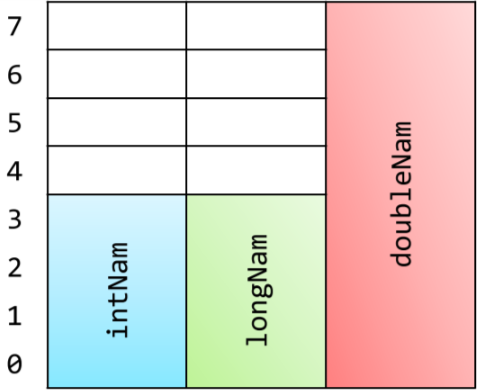
\includegraphics[width=\linewidth]{images/union.png}
\end{minipage}

\subsection{Bitfelder}

\subsubsection{Eigenschaften von Bitfeldern}
\begin{itemize}
	\item Innerhalb eines \emph{int} können einzelne Bitgruppen definiert und angesprochen werden.
	\item Sollte nicht eingesetzt werden, um damit Speicher zu sparen.
	\item Bei Embedded Systems ist der Einsatz unter Umständen sehr nützlich, wenn auf einzelne Register zugegriffen werden soll.
	\item[\-]\begin{achtung}
		Leider definiert der C++-Standard (und auch der C-Standard) nicht, ob die Bits von Links nach Rechts oder von Rechts nach Links aufgefüllt werden. Falls der Standard dies definieren würde, wären die Bitfelder ein sehr gutes Konstrukt.
	\end{achtung}
\end{itemize}

\subsubsection{Definition von Bitfeldern}
\vspace{-\baselineskip}
\begin{minipage}{\linewidth}
\begin{lstlisting}
struct FieldName
{
	unsigned int a: 3;	// definiert 3 Bits fuer a
	unsigned int b: 4;	// definiert die naechsten 4 Bits fue b
	...
};
\end{lstlisting}
\end{minipage}
\begin{minipage}{0.8\linewidth}
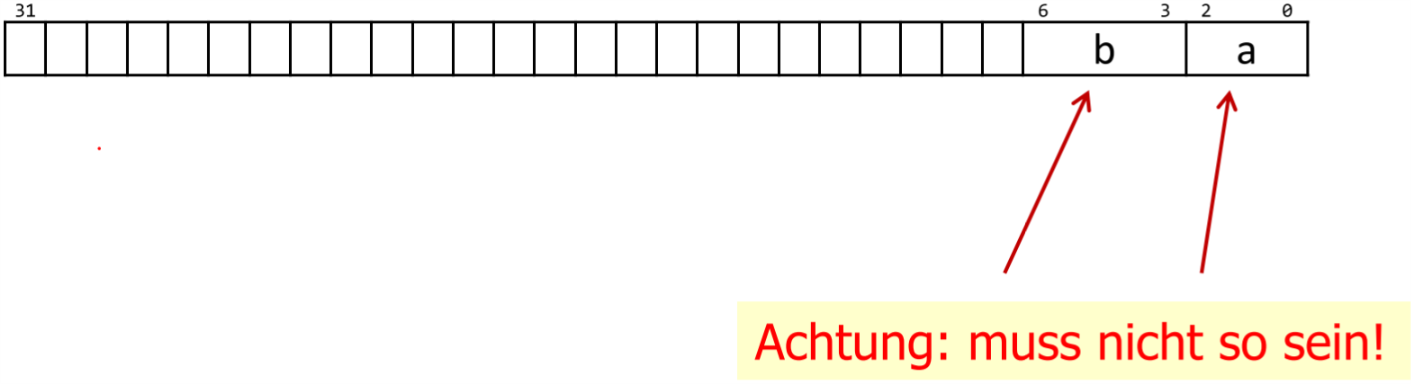
\includegraphics[width=\linewidth]{images/bitfelder.png}
\end{minipage}

\subsubsection{Bitfelder: Folgerungen}
\begin{itemize}
	\item Mit diesem Bitfeld-Mechanismus soll weder in C noch in C++ gearbeitet werden wenn der Code portabel sein soll.
	\item Die bessere Alternative ist die Verwendung von Bitmasken-Operationen. Diese können in C++ bspw. in inline-Funktionen verpackt werden.
\end{itemize}

%TODO weiter korrigieren

\subsection{Demo: Klasse Date}
Eine Klasse zur Speicherung und Darstellung von Kalenderdaten, wie z.B. 17.4.2013

%%% Datei einfügen %%%




%%% Complex Folien einfügen %%%